\paragraph{Game}

\begin{enumerate}

\item {\bf A 3-Player Game Tree} 

Consider the 3-player game shown below.  The player going first (at the top
of the tree) is the Left player, the player going second is the Middle
player, and the player going last is the Right player, optimizing the
left, middle and right components respectively of the utility vectors shown.   Fill in the
values at all nodes.  Note that all players \emph{maximize} their
own respective utilities.

\begin{center}
    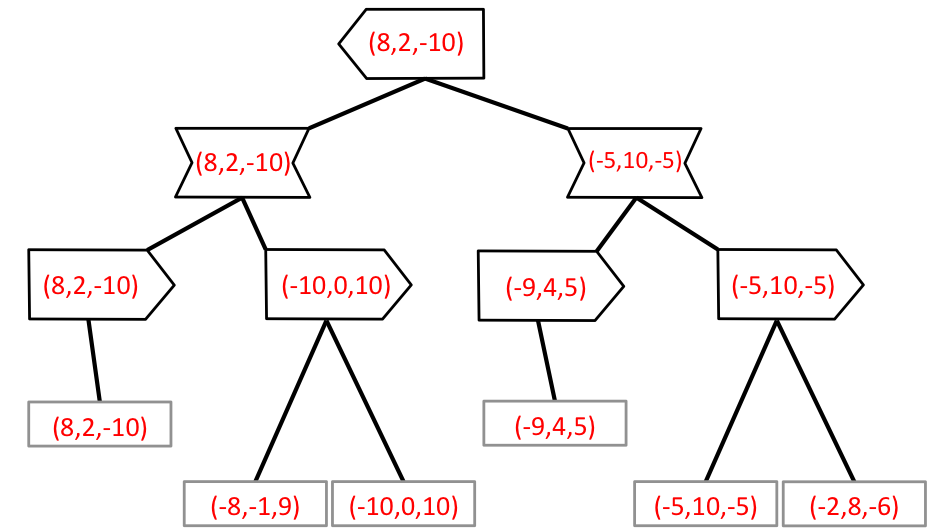
\includegraphics[width=5in]{figures/abg_solution}
\end{center}

\vspace{1cm}


\item {\bf Pruning for a 3-Player Zero-Sum Game Tree}

We would like to prune nodes in a fashion similar to $\alpha$ - $\beta$ pruning.  Assume that we have the knowledge that the sum of the utilities of all 3 players is always zero.
What pruning is possible under this assumption?  Below, cross off with an $\times$ any branches that can be safely pruned.   If no branches can be pruned, justify why not:

\begin{center}
     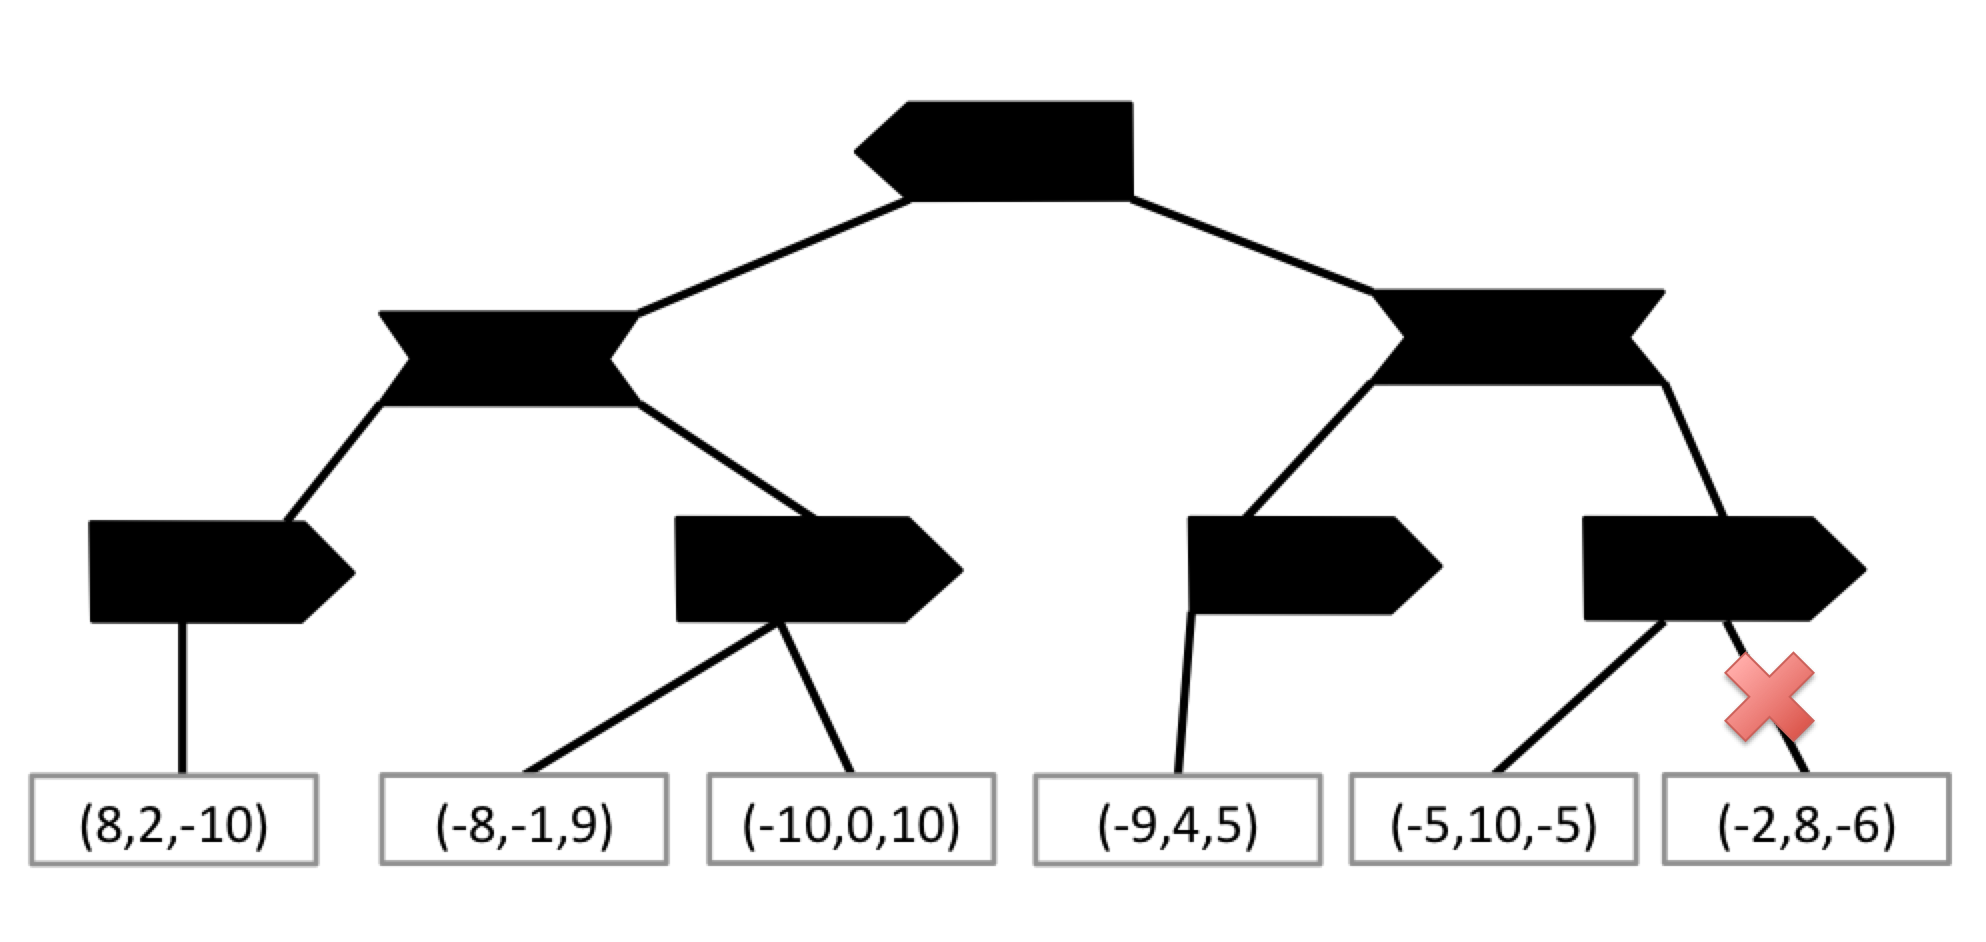
\includegraphics[width=4in]{figures/solution_b}
\end{center}

{\color{red}
The node farthest on the right can be pruned.
This is because by the time search reaches this node, we know that the first player can achieve a utility of 8, the second player can achieve a utility of 4, and the third player can achieve a utility of -5.
Since the game is required to be a zero-sum game and the sum of these utilities is 7, we know that there can be no possible node remaining in the tree which all players will find preferable to their current outcomes, and so we can prune this part of the tree.
}


\item {\bf Pruning for a 3-Player Zero-Sum, Bounded-Utility Game Tree.}

If we assume more about a game, additional pruning may become possible.  Now, in addition to assuming that the sum of the utilities of
all 3 players is still zero, we also assume that all utilities are in the interval $[-10, 10]$.
What pruning is possible under these assumptions?  Below, cross off with an $\times$ any branches that can be safely pruned.   If no branches can be pruned, justify why not:

\begin{center}
    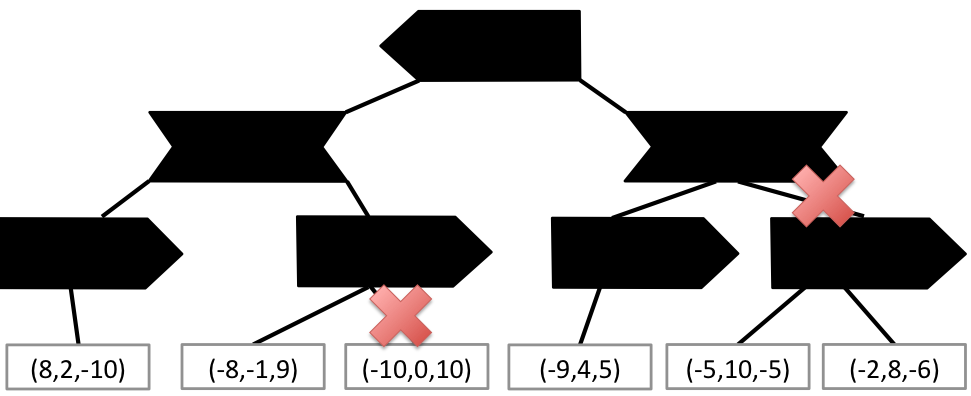
\includegraphics[width=4in]{figures/skeleton_solution}
\end{center}

{\color{red}
Pruning is now possible, for which we can bound the best case scenario for the player above us.

For the first pruning at $(-10,0,10)$, the Right player sees a value of 9. This means that Right can get at least a 9, no matter what other values are explored next. If Right gets a 9, then Middle can only get at best a 1 (calculated from $C - v_R = 10 - 9$), which corresponds to the utility triple $(-10,1,9)$.

Middle however has an option for a 2 above, so Middle would never prefer this branch so we can prune.

Similar reasoning holds for the pruning on the right -- Middle sees a 4, which means Left would get at best a 6, but Left already has an option for an 8, so all other parts of this tree will never be returned upwards.
    }

\end{enumerate}